Сначала измерим число частиц без поглотителя: $\langle N_0 \rangle \approx
175000$ частиц за $30$ секунд. Теперь перекроем колимматорный канал толстой
свинцовой пробкой. Результаты измерений за 30 секунд представлены в таблице
ниже.

\begin{table}[h!]
  \centering
  \caption{Измерение фона}
  \import{./src/tex_tbl/}{Back.tex}
\end{table}

Теперь проведем измерения, закрывая колимматорный канал поглотителями разной
толщины и из разных веществ. Таблицы с результатами измерений, а также
соответствующие графики представлены ниже. ($N_P = \langle N \rangle
-N_{\text{Ф}}$)
\newpage
\begin{figure}[h!]
  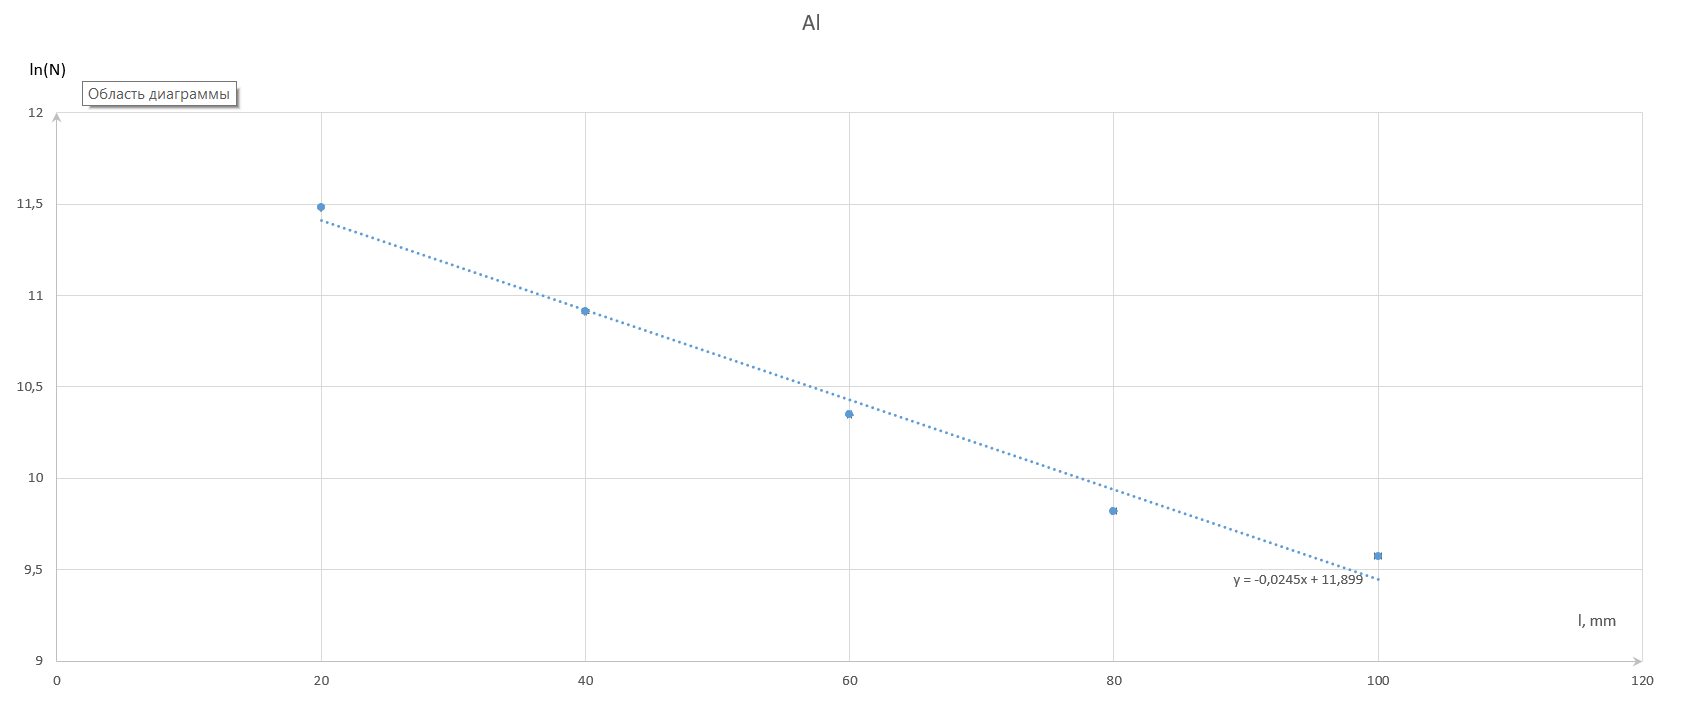
\includegraphics[width=\linewidth]{Al.png}
  \caption{График зависимости $\ln{(\langle N \rangle-N_{\Phi})}$ от $l$
  (Алюминий).}
\end{figure}

\begin{table}[h!]
  \centering
  \caption{Измерения для алюминия}
  \import{./src/tex_tbl/}{Al.tex}
\end{table}

\newpage
\begin{figure}[h!]
  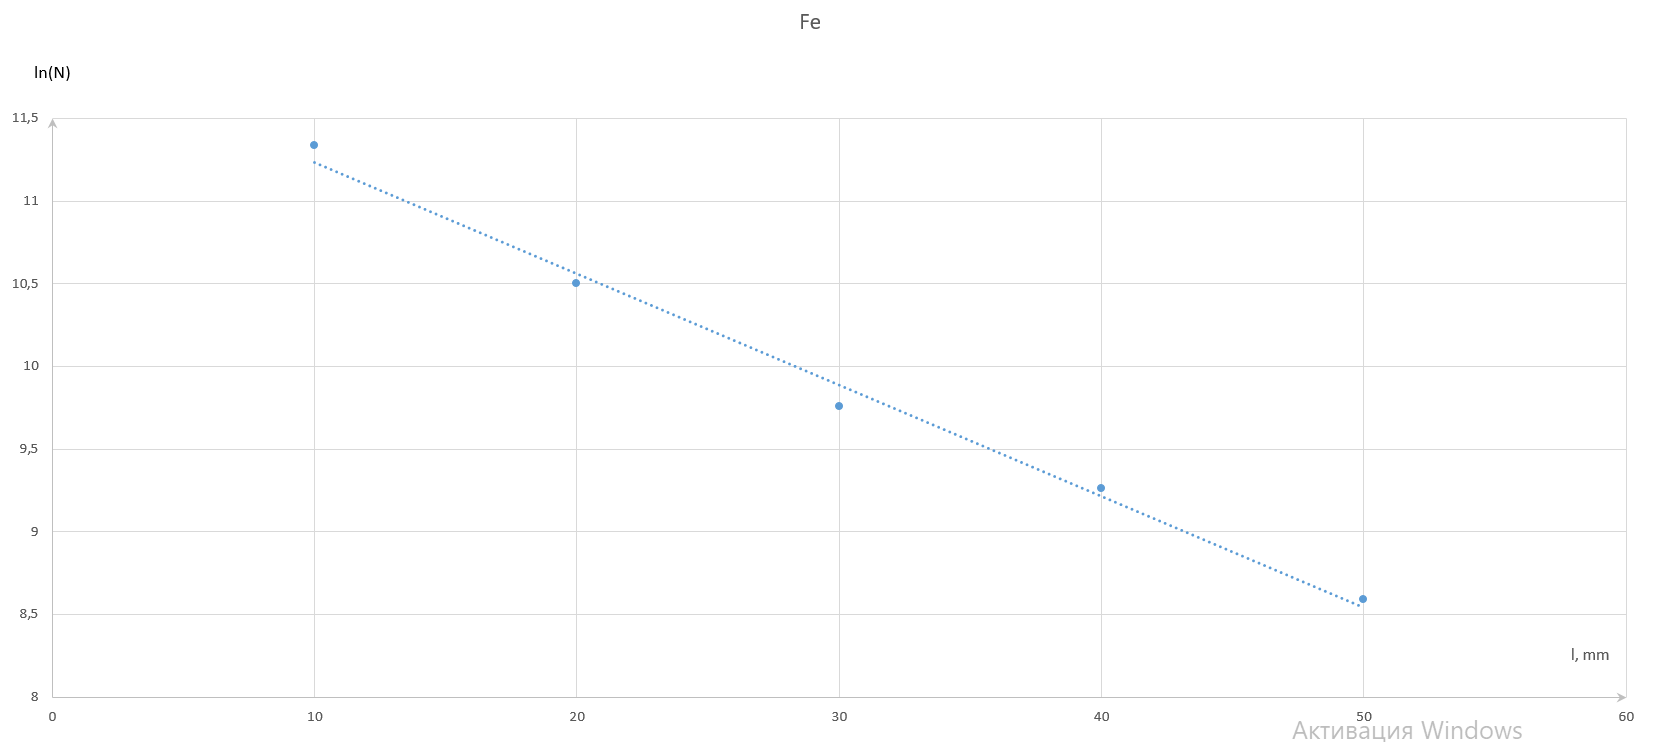
\includegraphics[width=\linewidth]{Fe.png}
  \caption{График зависимости $\ln{(\langle N \rangle-N_{\Phi})}$ от $l$
  (Железо).}
\end{figure}

\begin{table}[h!]
  \centering
  \caption{Измерения для железа}
  \import{./src/tex_tbl/}{Fe.tex}
\end{table}

\newpage
\begin{figure}[h!]
  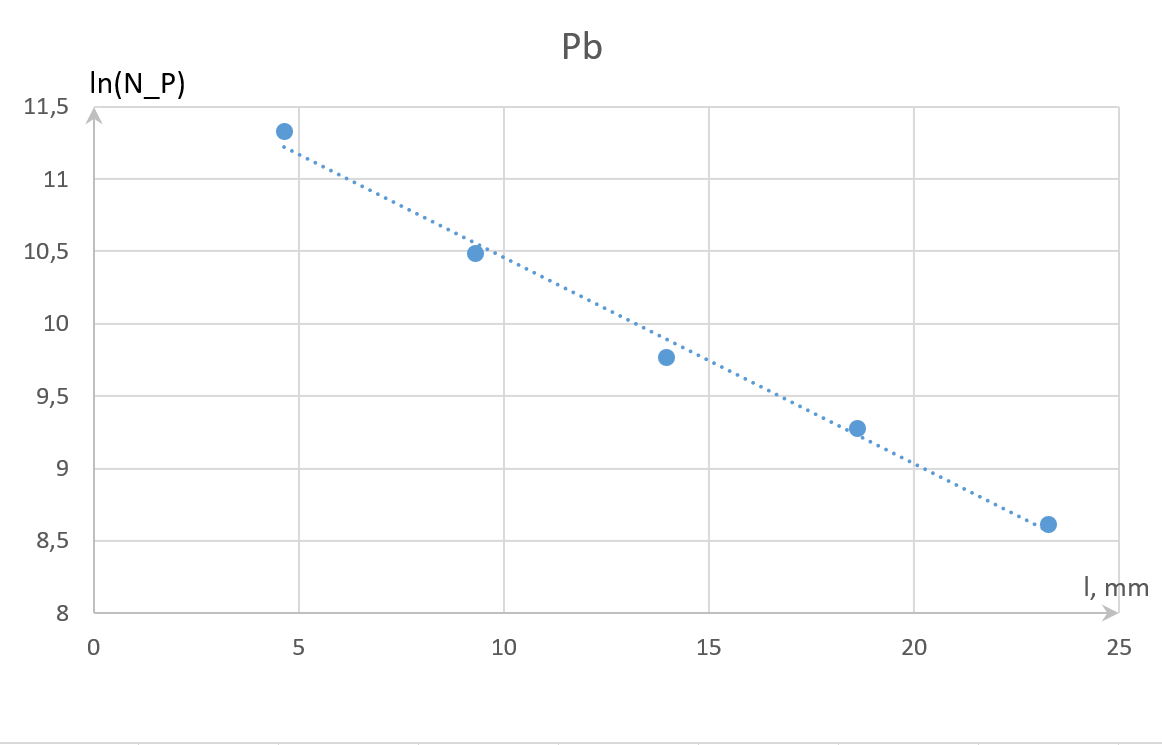
\includegraphics[width=\linewidth]{Pb.png}
  \caption{График зависимости $\ln{(\langle N \rangle-N_{\Phi})}$ от $l$
  (Свинец).}
\end{figure}

\begin{table}[h!]
  \centering
  \caption{Измерения для свинца}
  \import{./src/tex_tbl/}{Pb.tex}
\end{table}

\newpage
\begin{figure}[h!]
  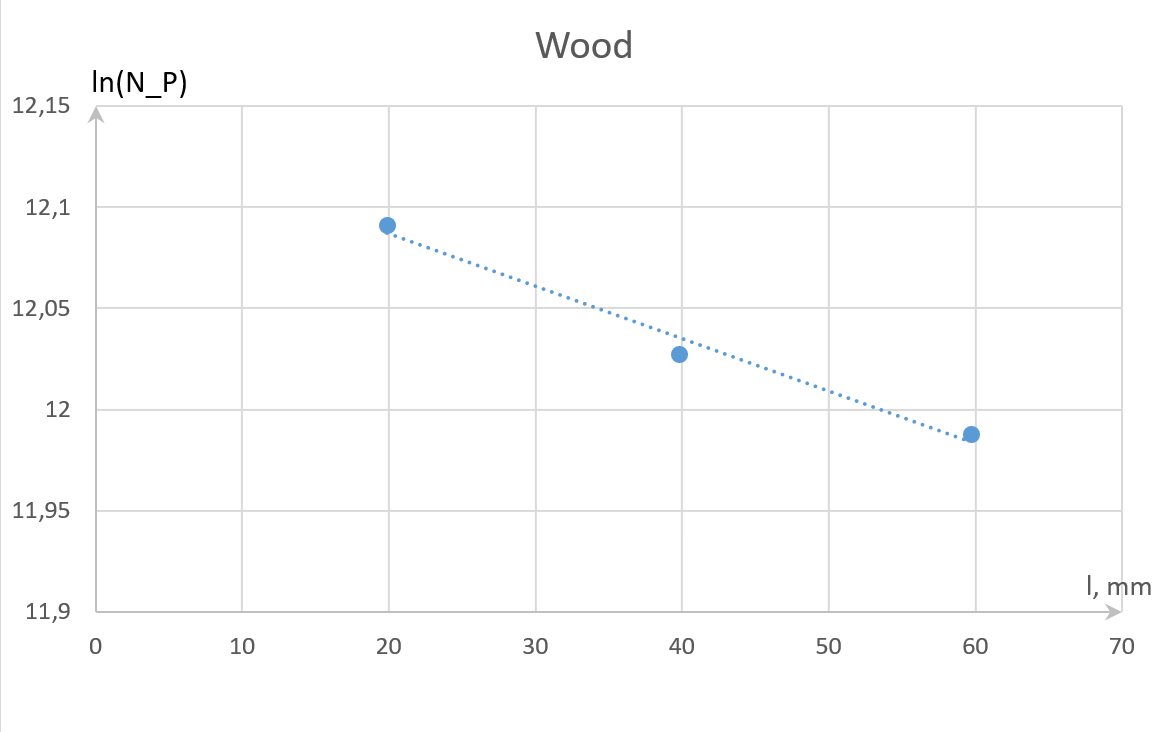
\includegraphics[width=\linewidth]{Wood.png}
  \caption{График зависимости $\ln{(\langle N \rangle-N_{\Phi})}$ от $l$
  (Дерево).}
\end{figure}

\begin{table}[h!]
  \centering
  \caption{Измерения для дерева}
  \import{./src/tex_tbl/}{Wood.tex}
\end{table}


Для каждого графика рассчитаем коэффициент наклона по МНК, занесём результаты в
таблицу:

\newpage

\begin{table}[h!]
  \centering
  \caption{Результаты}
  \import{./src/tex_tbl/}{result.tex}
\end{table}

Из справочных данных в лабораторном практикуме табличное значение энергии для
энергии алюминия -- $0.4$ МэВ, для железа -- $0.6$ МэВ, свинца -- $0.5$ МэВ.
Таким образом, средняя энергия $\gamma$-квантов равна $0.5$ МэВ.
